\begin{frame}
    \begin{centering}
        \vskip5ex plus 1filll
        {\usebeamerfont{title page title}\usebeamercolor[fg]{title page} Wavefolding\\[1.5ex]}
        \vskip0pt plus 1filll
    \end{centering}
\end{frame}

\begin{frame}{Wavefolder}
    What is wavefolding?
    \begin{figure}
        \centering
        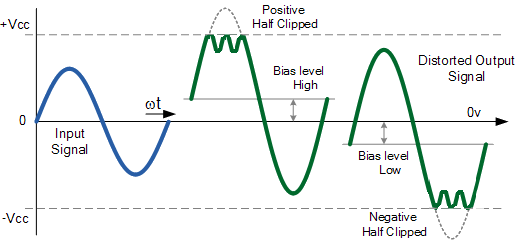
\includegraphics[width=4.5in]{Figures/wavefold.png}
    \end{figure}
\end{frame}

\begin{frame}{Wavefolder}
    Standard digital wavefolding:
    \vspace{2ex}
    \begin{columns}
        \begin{column}{0.5\linewidth}
            $f_{NL}(x) = sin(x)$
            \vspace{-3ex}
            \begin{figure}
                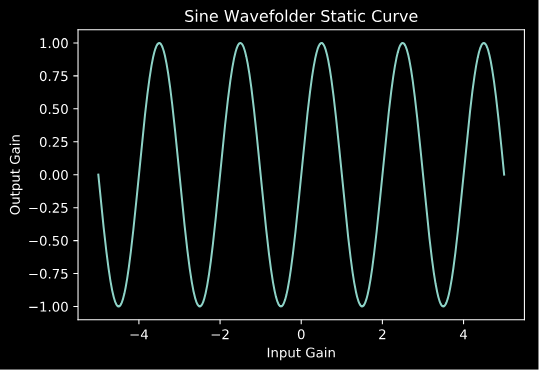
\includegraphics[height=2in]{../Wavefolder/Pics/sine_static}
            \end{figure}
        \end{column}
        \begin{column}{0.5\linewidth}
            $f_{NL}(x) = tri(x)$
            \vspace{-3ex}
            \begin{figure}
                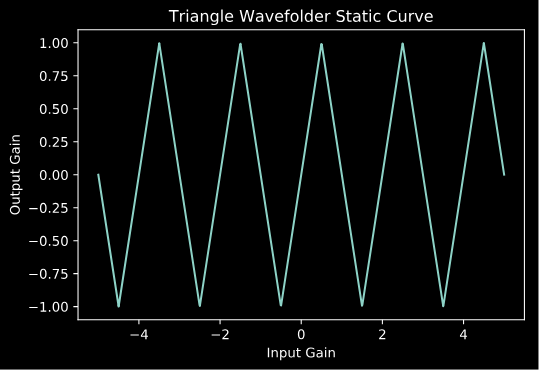
\includegraphics[height=2in]{../Wavefolder/Pics/tri_static}
            \end{figure}
        \end{column}
    \end{columns}
\end{frame}

\begin{frame}{Wavefolder}
    Standard digital wavefolding:
    \begin{figure}
        \centering
        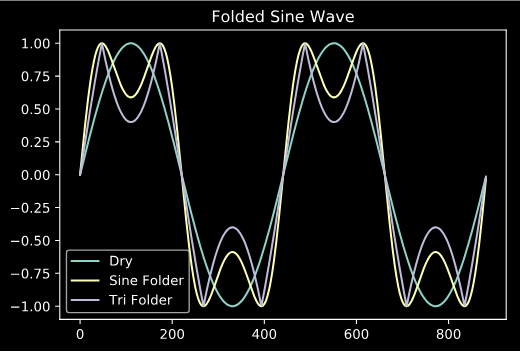
\includegraphics[height=2.5in]{../Wavefolder/Pics/simple_fold}
    \end{figure}
\end{frame}

\begin{frame}{Wavefolder}
    Saturating wavefolder:
    \begin{figure}
        \centering
        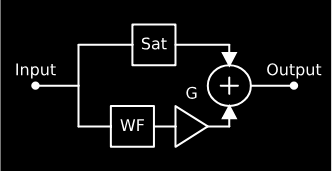
\includegraphics[width=4in]{../Wavefolder/Pics/sat_arch}
    \end{figure}
\end{frame}

\begin{frame}{Wavefolder}
    Saturating wavefolder:
    \begin{figure}
        \centering
        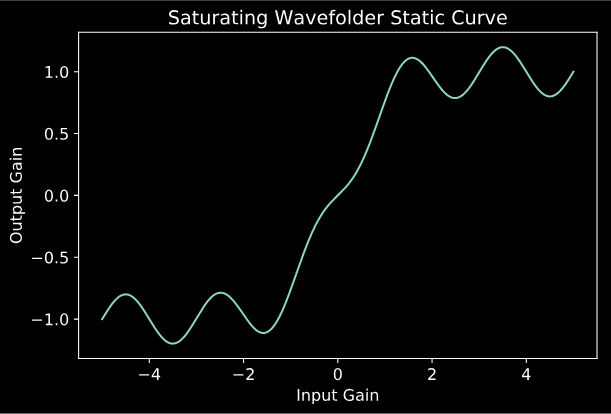
\includegraphics[height=2.5in]{../Wavefolder/Pics/sat_static}
    \end{figure}
\end{frame}

\begin{frame}{Wavefolder}
    Saturating wavefolder:
    \begin{figure}
        \centering
        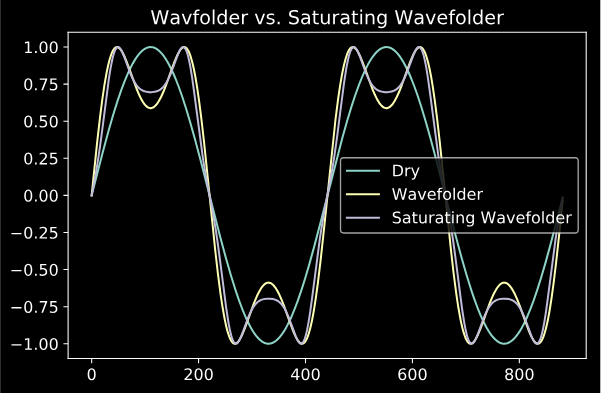
\includegraphics[height=2.5in]{../Wavefolder/Pics/sat_wave}
    \end{figure}
\end{frame}

\begin{frame}{Wavefolder}
    Saturating wavefolder:
    \begin{figure}
        \centering
        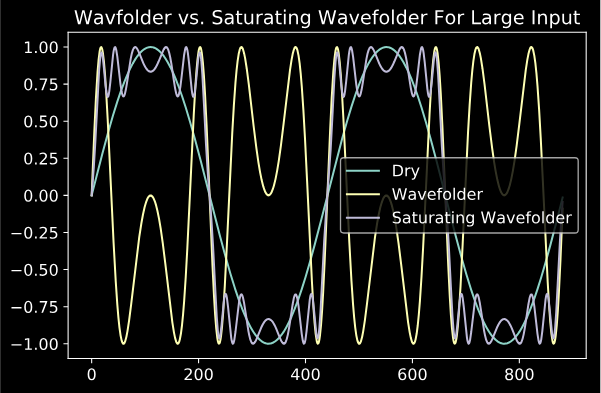
\includegraphics[height=2.5in]{../Wavefolder/Pics/sat_wave_large}
    \end{figure}
\end{frame}

\begin{frame}{Wavefolder}
    Feedback wavefolder:
    \begin{figure}
        \centering
        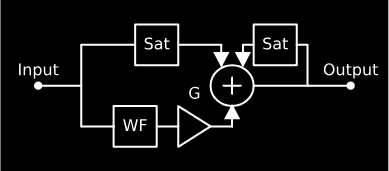
\includegraphics[width=4in]{../Wavefolder/Pics/fb_arch}
    \end{figure}
\end{frame}

\begin{frame}{Wavefolder}
    Feedback wavefolder:
    \begin{figure}
        \centering
        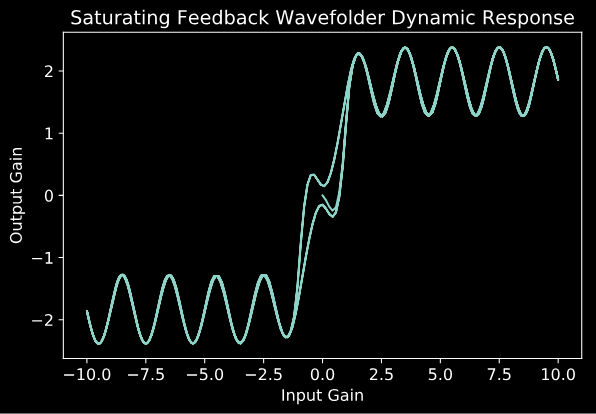
\includegraphics[height=2.5in]{../Wavefolder/Pics/fb_dyn}
    \end{figure}
\end{frame}
